\section{Evaluation}
\label{sec:sec_experiment}
In this section, we have evaluated accuracy and efficiency of our implementation
for People Counting problem. Because video can be considered as a sequence of
images, and counting people in a video is equivalent to summing on people
appearance in all frames of the video, the accuracy test is done at frame-level
using INRIA Dataset~\cite{2005_CVPR_Dalal}. For efficiency test, we examined the
execution time of our implementation against some large videos.

Our experiment is ran on SoC Tembusu cluster which contains 8 nodes of 16
Intel Xeon E5620 2.4GHz cores and equipped with 24GB memory. All 8 nodes shared
same 120GB disk. We used HDFS (Hadoop 1.2.1) as underlying storage and Apache
Spark 0.9.1 as execution engine. For video processing toolboxes, we used ffmpeg
4.2.1 and MATLAB R2012a.

\subsection{Accuracy Test}
\subsubsection{Dataset}
In this paper, we use INRIA Dataset for model training and accuracy testing. 
The INRIA Dataset~\cite{2005_CVPR_Dalal} was collected under the project LEAR.
The INRIA Dataset contains 2666 color images, in which the author cropped 1774
images of humans from a varied set of personal photos settings. The cropped
images were normalized into size of 64 $\times$ 128 pixels. The people are
usually standing, but appear in any orientation and against a wide variety of 
background image including crowds. Many are bystanders taken from the image
backgrounds, so there is no particular bias on their poses. Negative images are
collected to contain a diverse of scenarios including indoor, outdoor, mountain,
city and beach scenes. Some images also focus on cars, bicycles, motorbikes,
furniture, \etc.
% add figure
Examples images are shown in~\fig\ref{fig:inria_dataset_example}.
INRIA Dataset also suffers from selection bias, because the manual selection of
images from photographs. It is worthwhile to mention that INRIA Datast has
fairly high resolution pedestrians, while most data sets gather from mobile
platform have median heights that ranges from 50 - 100
pixels~\cite{2012_PAMI_Dollar}. The INRIA Dataset helped driven the recent
advances of pedestrian detection. In spite of its limitations, it remains as one
of the most popular pedestrian detection data sets. 

\begin{figure*}[!htbp]
  \centering

	\begin{minipage}{2.0\columnwidth}
	  \begin{minipage}{0.1\columnwidth} \centerline{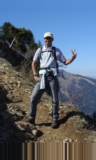
\includegraphics[width=1.05\linewidth]{inria_dataset/per00001}}  \end{minipage} \hfill 
	  \begin{minipage}{0.1\columnwidth} \centerline{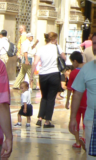
\includegraphics[width=1.05\linewidth]{inria_dataset/per00002}}  \end{minipage} \hfill 
	  \begin{minipage}{0.1\columnwidth} \centerline{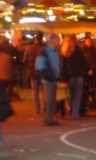
\includegraphics[width=1.05\linewidth]{inria_dataset/per000012}}  \end{minipage} \hfill 
	  \begin{minipage}{0.1\columnwidth} \centerline{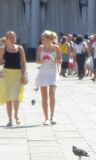
\includegraphics[width=1.05\linewidth]{inria_dataset/per00004}}  \end{minipage} \hfill 
	  \begin{minipage}{0.1\columnwidth} \centerline{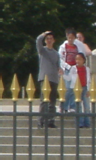
\includegraphics[width=1.05\linewidth]{inria_dataset/per00005}}  \end{minipage} \hfill 
	  \begin{minipage}{0.1\columnwidth} \centerline{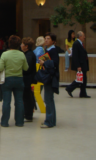
\includegraphics[width=1.05\linewidth]{inria_dataset/per00006}}  \end{minipage} \hfill 
	  \begin{minipage}{0.1\columnwidth} \centerline{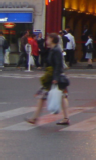
\includegraphics[width=1.05\linewidth]{inria_dataset/per00007}}  \end{minipage} \hfill 
	  \begin{minipage}{0.1\columnwidth} \centerline{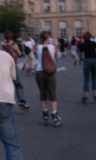
\includegraphics[width=1.05\linewidth]{inria_dataset/per00008}}  \end{minipage} \hfill 
	  \begin{minipage}{0.1\columnwidth} \centerline{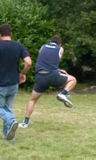
\includegraphics[width=1.05\linewidth]{inria_dataset/per00009}}  \end{minipage} \hfill
	\end{minipage}

    \begin{minipage}{2.0\columnwidth}
      \begin{minipage}{0.1\columnwidth} \centerline{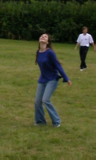
\includegraphics[width=1.05\linewidth]{inria_dataset/per000011}}  \end{minipage} \hfill 
      \begin{minipage}{0.1\columnwidth} \centerline{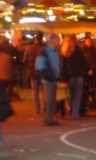
\includegraphics[width=1.05\linewidth]{inria_dataset/per000012}}  \end{minipage} \hfill 
      \begin{minipage}{0.1\columnwidth} \centerline{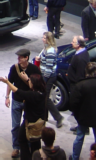
\includegraphics[width=1.05\linewidth]{inria_dataset/per000013}}  \end{minipage} \hfill 
      \begin{minipage}{0.1\columnwidth} \centerline{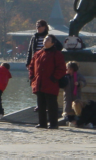
\includegraphics[width=1.05\linewidth]{inria_dataset/per000014}}  \end{minipage} \hfill 
      \begin{minipage}{0.1\columnwidth} \centerline{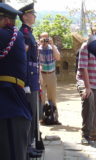
\includegraphics[width=1.05\linewidth]{inria_dataset/per000015}}  \end{minipage} \hfill 
      \begin{minipage}{0.1\columnwidth} \centerline{
\includegraphics[width=1.05\linewidth]{inria_dataset/per000016}}  \end{minipage} \hfill 
      \begin{minipage}{0.1\columnwidth} \centerline{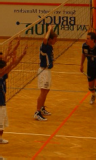
\includegraphics[width=1.05\linewidth]{inria_dataset/per000017}}  \end{minipage} \hfill 
      \begin{minipage}{0.1\columnwidth} \centerline{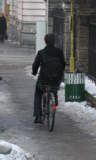
\includegraphics[width=1.05\linewidth]{inria_dataset/per000018}}  \end{minipage} \hfill 
      \begin{minipage}{0.1\columnwidth} \centerline{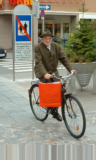
\includegraphics[width=1.05\linewidth]{inria_dataset/per000019}}  \end{minipage} \hfill
    \end{minipage}
    
  \vspace{-1ex}
  \caption
    {
    \small
	Some normalized image windows from the INRIA static person detection
	dataset. Note the variations in pose. Most of images contain people standing or
	walking. Some images have people running, going downhill, bicycling, or playing.
    }
  \label{fig:inria_dataset_example}
\end{figure*}


\subsubsection{Evaluation Method}
\label{subsec:evaluation_method}
The detection performance is measured by the number of true positive (TP - the
number of desired foreground objects detected by the detector) and false
positive  (FP - the number of background patches wrongly detected as the object
of  interest) detections~\cite{2013_ICCV_Hamed}. A detection is considered as
false positive if the predicted  bounding box with correlation response higher than the detection
threshold does not contain the target object. A detection is true positive if 
the overlap ratio $a_0$ between the predicted bounding box $B_p$ and a ground
truth bounding box $B_{gt}$ is more than a decision threshold $\theta$,
\begin{equation}
	a_0 = \frac{area(B_p \cap B_{gt})}{area(B_p \cup B_{gt})} \geq \theta
\end{equation}
The trade-off between TP and FP can be effectively measured using detection
rate versus false positive rate, Precision-Recall and Recall-FPPI  (false
positive per image) by varying a threshold and computing the recall and
precision/FPPI  for each threshold value, where
\begin{equation}
	Recall = \frac{TP}{nP}
\end{equation}

\begin{equation}
	Precision = \frac{TP}{TP + FP}
\end{equation}

\begin{equation}
	FPPI = \frac{FP}{N}
\end{equation}
where TP, nP, FP and N respectively indicate the true positive detections, the
total number of desired objects, the number of false detections and the number of test images.


\subsubsection{Experiment Accuracy Comparison}
The goal of experiment of accuracy comparison is to compare the performance of
person detection in standalone computer and computer clusters. In the
experiment, the person detector is trained using INRIA Dataset which is
described above. The testing data is also from from the same dataset which
consists of 288 images possible containing persons inside. 

After detection, we will get some bounding box locations for each image.
Combining detection results and ground truth information from INRIA Dataset.
We apply the evaluation in~\ref{subsec:evaluation_method} to get the
performance evaluation results. We plot the ROC(Receiver Operating
Characteristic) curve of the result.
The result is shown in~\fig\ref{fig:inria_roc}. As can be seen
in~\fig\ref{fig:inria_roc}, the detection result is same by performing HOG
method~\cite{2005_CVPR_Dalal} on standalone computer and computer clusters. The
slight different is result from some executing failure in the clusters. Thus
some testing images lack of the detection result. 

The result is of our expectation since we use same algorithm and also the same
implementation. The only difference is that the original implementation is
slightly modified so that it can be run on top of computer clusters to utilize
the computation power. 


\begin{figure}[!t]
  \centering
  \begin{minipage}{1.0\columnwidth}
  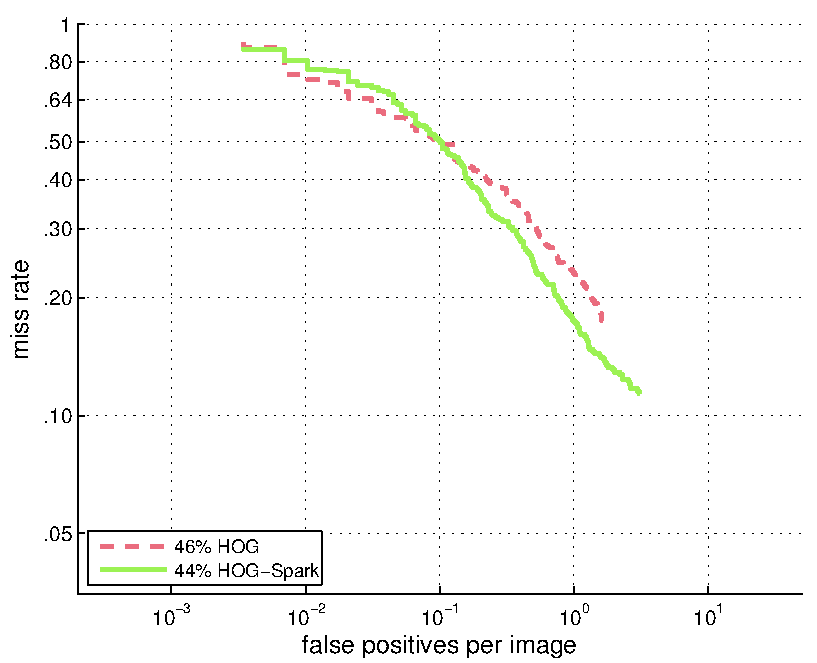
\includegraphics[width=1.05\linewidth]{InriaTest}
  \end{minipage}
  
  \vspace{-1ex}
  \caption
    {
    \small
	Results on INRIA Dataset with same detector running using standalone machine
	and computer clusters. The resulting performance is almost same as illustrated
	in the figure. }
  \label{fig:inria_roc}
\end{figure}

\subsection{Efficiency Test}
We intended to evaluate scalability of our implementation by executing at
different cluster size: 1, 2, 4 and 8. However, we could not make HDFS run
successfully on Tembusu cluster because all 8 nodes shared same logical disk
view. Parallel and distributed programs which designed for running at large
scale, such as MPI, Hadoop MapReduce, Spark, often have a uniform setup for all
workers, i.e. all nodes have same directory structure, for automation and
ease of management. Tembusu cluster setup works well when application only read
input data for processing and there is only one master responsible for writing
output. Our Spark application involves a lot read and write between
execution phases which resulted in only 1 datanode have privilege to access data
in order to avoid data race problem. Therefore, we can only use 2 nodes for our
experiment: 1 master node and 1 worker node with 4 worker threads (to have
sufficient memory for each task).

For efficiency test, we run our People Counting program with a 262MB surveillance
video which contains 6154 frames. Our program took 3225 second to complete the
job and the degree of parallelism is 4 (4 worker threads). Compare to processing
frame by frame, it would take around 6154 frame x 11.5 second/frame (the mean
frame execution time taken from accuracy test) which is 70771 second. Ignore
parallel overhead, frame execution could take about 17692 second to finish. The
source of improvement is coarse-grain execution by using GOP as computation unit
instead of frame and less number of MATLAB call. Although this is not a totally
fair comparison, it can show the promise of using big data frame work to speed
up video processing time.
